% Constelação 16-QAM com rótulos de Gray e um ponto recebido com ruído.
\begin{figure}[!htb]
\centering
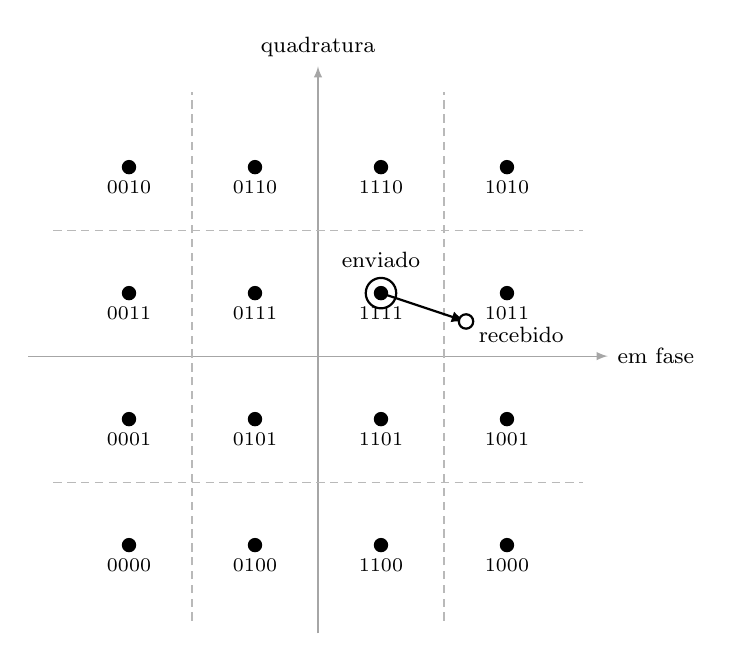
\begin{tikzpicture}[x=0.8cm,y=0.8cm,font=\footnotesize,>=latex]
  % eixos
  \draw[->,gray!70] (-4.6,0) -- (4.6,0) node[right,black] {em fase};
  \draw[->,gray!70] (0,-4.4) -- (0,4.6) node[above,black] {quadratura};
  % fronteiras de decisão
  \foreach \v in {-2,2}{
    \draw[densely dashed,gray!55] (\v,-4.2) -- (\v,4.2);
    \draw[densely dashed,gray!55] (-4.2,\v) -- (4.2,\v);}
  % pontos em código de Gray: amplitude -> rótulo de 2 bits
  \def\lab#1{\ifcase#1 00\or 01\or 11\or 10\fi}
  \foreach \i/\x in {0/-3,1/-1,2/1,3/3}{
    \foreach \j/\y in {0/-3,1/-1,2/1,3/3}{
      \fill (\x,\y) circle (2.6pt);
      \node[below=1.5pt,font=\scriptsize] at (\x,\y) {\lab{\i}\lab{\j}};
    }}
  % ponto enviado, ponto recebido com ruído e o erro
  \draw[black,thick] (1,1) circle (5.5pt);
  \node[anchor=south,fill=white,inner sep=1pt] at (1,1.36) {enviado};
  \draw[->,thick] (1,1) -- (2.35,0.55);
  \fill[white,draw=black,thick] (2.35,0.55) circle (2.6pt);
  \node[anchor=north west,inner sep=1pt] at (2.5,0.52) {recebido};
\end{tikzpicture}
\caption{16-QAM: cada ponto representa 4 bits. As linhas tracejadas são as
fronteiras de decisão. Aqui \texttt{1111} é enviado, o ruído empurra a medida
para além de uma fronteira, e o receptor decide \texttt{1011}. Como os rótulos
seguem um código de Gray, pontos vizinhos diferem em um único bit.}
\label{fig:qam}
\end{figure}
